\title{Problem Set III}
\author{
  Ethan Rooney
}
\date{\today}

\documentclass[12pt]{article}
\usepackage{amssymb}
\usepackage{amsmath}
\usepackage{cancel}
\usepackage{graphicx}
\usepackage[margin=1in]{geometry}

\begin{document}
\maketitle

\section{Problem 1}
Tayler expansion of $e^{-iqr}V(r)$

\begin{equation}
  \frac{df}{dr'}=-iqe^{-iqr'}V(r')+\frac{dV}{dr'}(r')e^{-iqr'}
\end{equation}

\begin{equation}
  \frac{d^2f}{dr'^2}= (-iq)^2e^{-iqr'}V(r') + \frac{dV}{dr'}(r')e^{-iqr'} - (iq)\frac{dV}{dr'}(r')e^{-iqr'} + \frac{d^2V}{dr'^2}(r')e^{-iqr'}  
\end{equation}

\begin{equation}
  f_{Taylor}(r,r'=0) \approx f(0)+f'(0)r= V(0)+[V(0)+\frac{dv}{dr}(0)]r
\end{equation}

When we substiture the given equation for $V(r)$ into the above

\begin{equation}
  f(\theta,\phi)=-\frac{m}{2\pi\hbar}[V_{0}2\pi{r_0}(1-iq-\frac{r_0^2}{4})]
\end{equation}

\begin{equation}
  |f(\theta,\phi)|^2=\frac{m^2r_0^2V_{0}^2}{\hbar^216}(16q^2+r^2-4)
\end{equation}

\section{Problem 2}

\begin{equation}
 k+p=k'+p' 
\end{equation}

\begin{equation}
  k+k'=p'- p
\end{equation}

\begin{equation}
  (k+k')^2=(p'- p)^2
\end{equation}

\begin{equation}
  \cancelto{0}{k^2}+\cancelto{0}{k'^2} -2k_{\mu}k^\mu=\cancelto{M}{p'^2}+\cancelto{M}{p^2} - 2p_\mu p'^\mu
\end{equation}

\begin{equation}
  -2k_{\mu}k^\mu= 2M - 2p_\mu p'^\mu
\end{equation}

\begin{equation}
  k_{\mu}k^\mu=  p_\mu p'^\mu -M
\end{equation}

\begin{equation}
   k=\langle E,0,0,E\rangle 
\end{equation}
\begin{equation}
   k'=\langle E',0,E'\sin\theta,E'\cos\theta\rangle 
\end{equation}
\begin{equation}
   p=\langle M,0,0,0\rangle 
\end{equation}
\begin{equation}
   p'=\langle M,0,-E\sin\theta,E-E\cos\theta\rangle 
\end{equation}

\begin{equation}
  EE'+EE'\cos\theta=M^2-M 
\end{equation}

\begin{equation}
  E'=\frac{M^2-M}{E(1+\cos\theta)}
\end{equation}

\section{Problem 3}

\begin{equation}
  N=\frac{d\sigma}{d\Omega} \cdot I \cdot \Omega \cdot\alpha\cdot t
\end{equation}

\begin{equation}
  t=\frac{N}{ \frac{\alpha^2\cos^2{\frac{\theta}{2}}}{E^2\sin^2{\frac{\theta}{2}} } \cdot I \cdot \Omega \cdot\alpha }
\end{equation}

When all values are subbed in I found:

\[
  t_{10^\circ} = 3.783251e+11 \mbox{ seconds}
\]
\[
  t_{30^\circ} = 3.129442e+13 \mbox{ seconds}
\]
\[
  t_{45^\circ} = 1.634924e+14 \mbox{ seconds}
\]
\[
  t_{60^\circ} = 5.422360e+14 \mbox{ seconds}
\]
\[
  t_{90^\circ} = 3.253416e+15 \mbox{ seconds}
\]
\[
  t_{170^\circ} = 8.436348e+17 \mbox{ seconds}
\]


\begin{figure}[h]
  \centering
  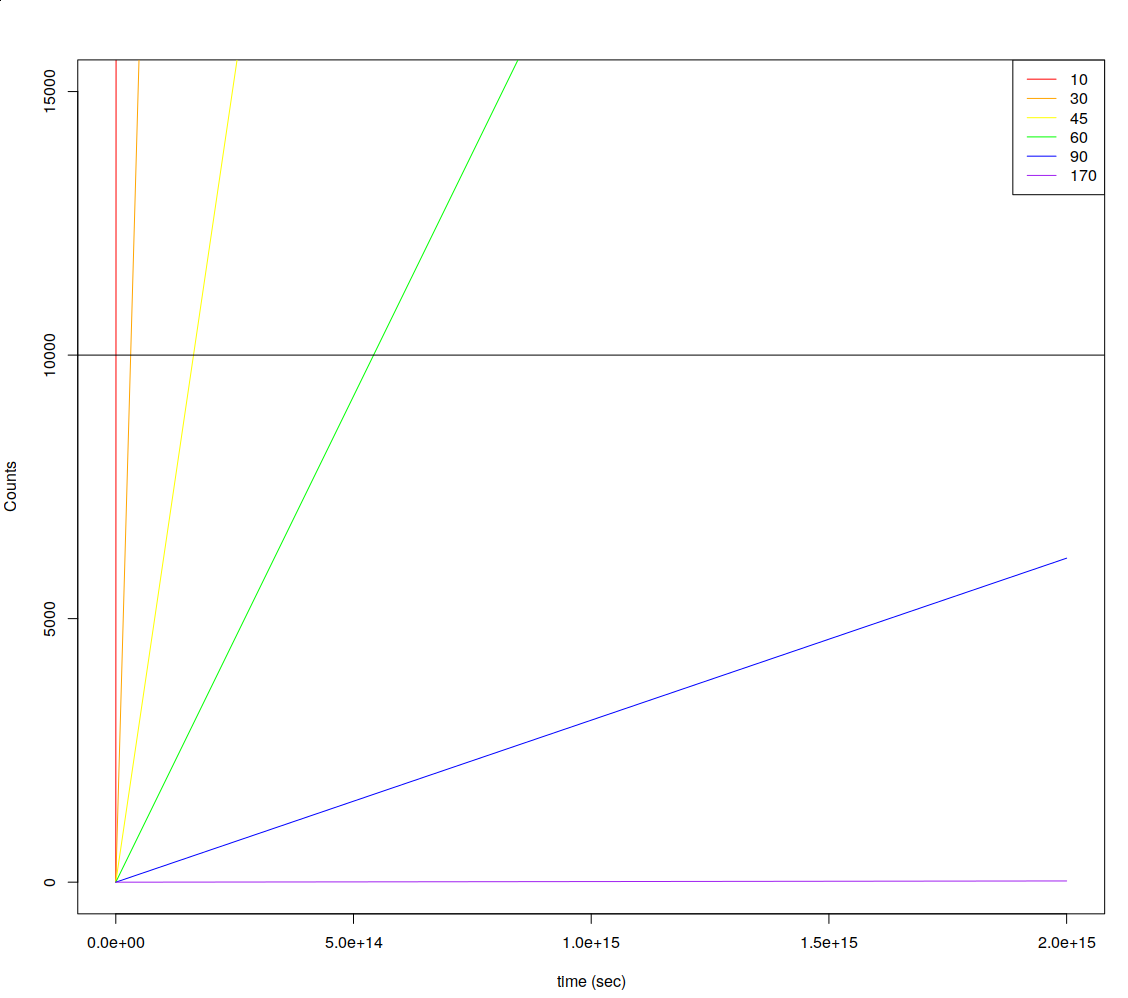
\includegraphics[width=300pt]{code/p3graph.png}
  \caption{Time to 10000 Counts for various scattering angles}
\end{figure}

\newpage

\section{Problem 4}

\begin{equation}
  F(q)=\int e^{-iqr}\rho(r)d^3r
\end{equation}

\begin{equation}
  F(q)= \int\int\int_0^f e^{-iqr}\rho_0r^2drd\cos\theta d\phi +\cancelto{0}{\int\int\int_r^\infty e^{-iqr}\rho(0)r^2drd\cos\theta d\phi }
\end{equation}

\begin{equation}
  F(q)= \rho_0 2\pi\int r^2\int e^{-iqr}d\cos\theta dr
\end{equation}

\begin{equation}
  F(q)= \rho_0 2\pi\int r * \frac{e^{-iqr\cos\theta}}{-iq}\rvert_{-1}^{1} dr
\end{equation}

\begin{equation}
  F(q)= \rho_02\pi\int \frac{2r}{q}\sin{qr} dr=\frac{4\pi\rho_0(\sin{qr}-qr\cos{qr})}{q^3}
\end{equation}


\begin{figure}[h]
  \centering
  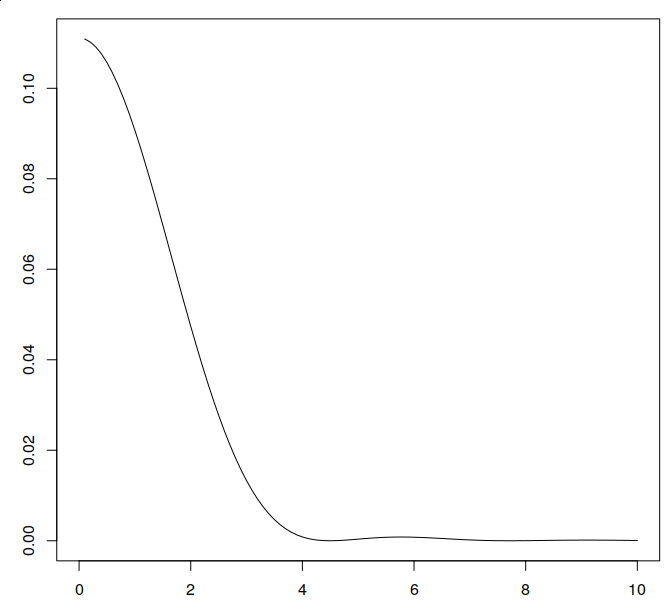
\includegraphics[width=300pt]{p4_form_factor.png}
  \caption{$|F(q)|^2$ for various momentum transfer}
\end{figure}

\newpage
\section{Problem 5}

To do 5, I used Pythons built in fast fourier transform. This let me read in the data from the provided file, and then perform the the transform on the data.

\begin{figure}[h]
  \centering
  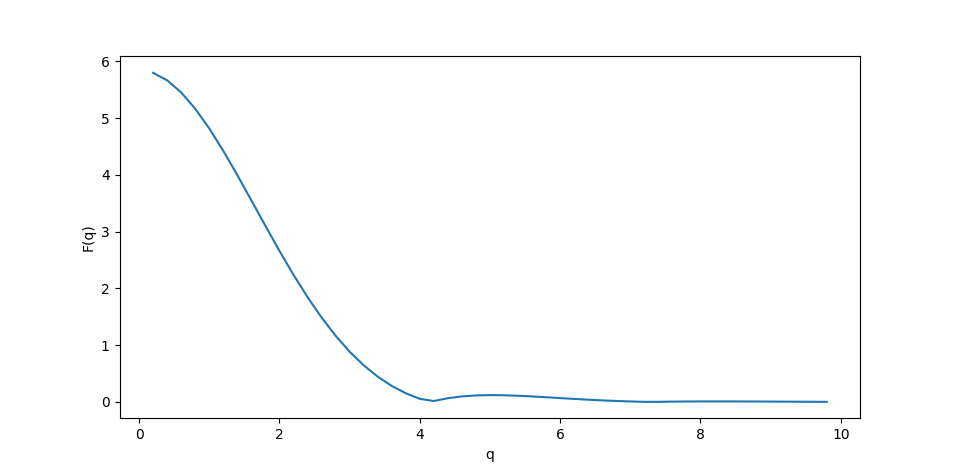
\includegraphics[width=400pt]{code/f_q.png}
  \caption{$F(q)$ for various momentum transfer}
\end{figure}

\begin{figure}[h]
  \centering
  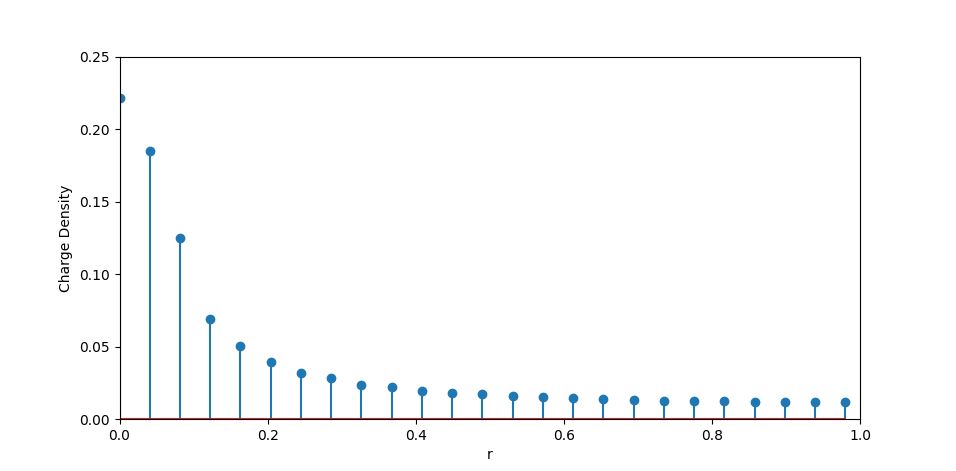
\includegraphics[width=400pt]{code/rho_r.png}
  \caption{$F(q)$ for various momentum transfer}
\end{figure}

\end{document}
